We recall several definitions from previous works of Cleve, Liu, Mittal, and Slofstra \cite{slofstra2016tsirelson,cleve2016perfect,cleve2014characterization}. Following a suggestion from \cite{cleve2016perfect}, we define the machinery over $\Z_d$ instead of $\Z_2$. %This doesn't require any fundamentally new ideas, but it allows us to analyze the games of interest. 
% The proofs from \cite{slofstra2016tsirelson,cleve2016perfect,cleve2014characterization} go through with almost no modifications, so we do not reproduce them here. (The interested reader need only make the modifications suggested at the end of Section 4 of \cite{cleve2016perfect}, and also add inverses to operators in the appropriate places.)
% This is not particularly interesting in its own right, but it allows us to analyze the games of interest.
% This gives us the first examples of natural games analyzed in the group-representation-theoretic framework, showing how these results greatly simplify self-testing proofs.


\begin{definition}
	A \emph{hypergraph} $\mathbf H = (V,E,H)$ consists of a finite \emph{vertex set} $V$, a finite \emph{edge set} $E$ and an \emph{incidence matrix} $H: V\times E \to \Z$. 
	% A hypergraph is called a (directed) \emph{graph} if every edge $e$ is supported on exactly two vertices and satisfies $\sum_v H(v,e) = 0$. 
	% A hypergraph is \emph{connected} if for every pair of vertices $(v,v')$ there is a \emph{path} $(v =v_0,e_1,v_1,\ldots e_k,v_k = v')$ such that each edge ``connects'' the two adjacent vertices, i.e.\ for all $1\leq i\leq k$, we have $H(v_i,e_i)\neq 0 \neq H(v_{i-1},e_{i})$. 
\end{definition}
We think of $V$ as a set of $\Z$-linear equations, $E$ as a set of variables, and $H(v,e)$ as the coefficient of variable $e$ in equation $v$. Following Arkhipov \cite{arkhipov2012extending}, some of our hypergraphs of interest will be graphs. Unlike previous works, we introduce signed coefficients (outgoing edges have a positive sign in the incidence matrix, while ingoing edges have a negative sign). This is because previous works considered equations over $\Z_2$, where $1 = -1$.
% We'll be especially interested in so-called ``magic games'': games which have a perfect strategy with some finite amount of entanglement, but which have no perfect strategy in the classical world.


\begin{definition}[\cite{cleve2014characterization}, \cite{slofstra2016tsirelson}]\label{definition:linear-constraint-game}
	Given hypergraph $\mathbf H$, vertex labelling $l: V \to \Z$, and some modulus $d\in \Z$, we can associate a nonlocal game which we'll call the \emph{linear constraint game} $\LCS(\mathbf H, l, \Z_d)$. Informally, a verifier sends one equation $x$ to Alice and one variable $y$ to Bob, demanding an assignment $a:E\to \Z_d$ to all variables from Alice and an assignment $b\in \Z_d$ to variable $y$ from Bob. The verifier checks that Alice's assignment satisfies equation $x \pmod d$, and that Alice and Bob gave the same assignment to variable $y$.
	\\\noindent
	Formally, we have the following question and answer sets: $X = V$, $Y = E$, $A = \Z_d^E$, $B = \Z_d$. The win condition selects those tuples $(a,b,x,y)$ satisfying:
	\begin{align}
	\label{eq:lcs-equation}
		a(y) &= b &&\text{(Consistency) }
	\\	\sum_{e\in E} H(x,e)a(e) &\equiv l(x) \pmod d.	&&\text{(Constraint satisfaction) }
	\end{align}
\end{definition}
We introduce the two primary LCS games of interest in this paper.
\begin{example}
\label{example:magic-square}
	The magic square LCS (mod $d$) has vertex set $\set{v_1,\ldots, v_6}$, edge set $\set{e_1,\ldots, e_9}$, vertex labeling $l(v_5) = 1, l(v_i) = 0$ for $i\neq 5$. See Figure \ref{fig:magic-square-equations} for the full description of the hypergraph and the associated set of linear equations.
	%, and incidence matrix given by 
	%\begin{align}
		%H(v_i,e_j) &= 1\text{ if }& (i,j) \in 
		%\{		&(1,1), (1,2), (1,3), (2,4), (2,5), 
		%\\&&	&(2,6),(3,7), (3,8), (3,9)\}
		%\\H(v_i,e_j) &= -1\text{ if }& (i,j) \in 
		%\{		&(4,1), (4,4), (4,7),(5,2), (5,5), 
		%\\&&	&(5,8), (6,3), (6,6), (6,9)\}.
	%\end{align}
	
\end{example}
\begin{figure}[h]
	\begin{center}
	\begin{multicols}{2}
	    \resizebox{0.2\textwidth}{!}{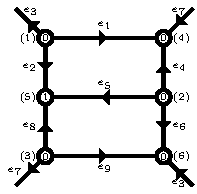
\includegraphics{MagicSquare-figure7.pdf}}
	    
	    \begin{align}
	    	(1)&& e_1 + e_2 + e_3 &= 0 & (4)&& -(e_1 + e_4 + e_7) &= 0 
	    \\	(2)&& e_4 + e_5 + e_6 &= 0 & (5)&& -(e_2 + e_5 + e_8) &= 1 
	    \\	(3)&& e_7 + e_8 + e_9 &= 0 & (6)&& -(e_3 + e_6 + e_9) &= 0 
	    \end{align}
	\end{multicols}
    \end{center}
    \caption{The magic square LCS, presented both in terms of equations (mod $d$) and in terms of a labelled hypergraph. The two line segments labeled $e_3$ are parts of the same edge, as are the pair of line segments labeled $e_7$. The underlying graph is $K_{3,3}$, the smallest bipartite non-planar graph. The direction of the edges emphasizes the bipartition.}
    \label{fig:magic-square-equations}
\end{figure}
\begin{example}
\label{example:magic-pentagram}
	The magic pentagram LCS (mod $2$) has vertex set $\set{v_1,\ldots, v_5}$, edge set $\set{e_1,\ldots, e_{10}}$, vertex labeling $l(v_5) = 1, l(v_i) = 0$ for $i\neq 5$. See Figure \ref{fig:magic-pentagram-equations} for the full description of the hypergraph and the associated set of linear equations.
\end{example}
\begin{figure}[h]
	\begin{center}
	\begin{multicols}{2}
	    \resizebox{0.3\textwidth}{!}{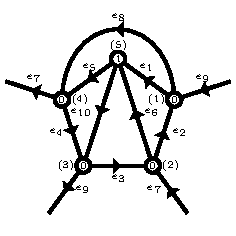
\includegraphics{MagicSquare-figure8.pdf}}

	    \begin{align}
	    (1)&& e_1 - e_2 + e_8 - e_9 	&= 0\\
	    (2)&& e_2 - e_3 + e_6 - e_7 	&= 0\\
	    (3)&& e_3 - e_4 + e_9 - e_{10} 	&= 0\\
	    (4)&& e_4 - e_5 + e_7 - e_{8} 	&= 0\\
	    (5)&& e_5 - e_6 + e_{10} - e_1 	&= 1\\
	    \end{align}
	\end{multicols}
    \end{center}
    \caption{The magic pentagram LCS, presented both in terms of equations (mod $2$) and in terms of a labelled hypergraph. The two line segments labeled $e_7$ are parts of the same edge, as are the pair of line segments labeled $e_9$. The underlying graph is $K_5$, the smallest complete non-planar graph.} 
    \label{fig:magic-pentagram-equations}
\end{figure}

The following is the main tool we use to understand linear constraint system games.

\begin{definition}[Solution group over $\Z_d$, \cite{cleve2016perfect}]
	For an LCS game $\LCS(\mathbf H, l, \Z_d)$ with $\mathbf H = (V,E,H)$, the \emph{solution group} $\G(\mathbf H, l, \Z_d)$ has one generator for each edge of $\mathbf H$ (i.e.\ for each variable of the linear system), one relation for each vertex of $\mathbf H$ (i.e.\ for each equation of the linear system), and relations enforcing that the variables in each equation commute. Formally, define the sets of relations $R_c$, the local commutativity relations, and $R_{eq}$, the constraint satisfaction relations as
	\begin{align}
		R_{c} 		&:= \set{[e,e'] \; H(v,e) \neq 0 \neq H(v,e')\text{ for some } v\in V}
		\\R_{eq}	&:= \set{ J^{-l(v)}\prod_{e\in E}e^{H(v,e)} \; v\in V}.
	\end{align}
Then define the solution group as
\begin{equation}
	\G(\mathbf H, l, \Z_d) := \Braket{E:R_{c}\cup R_{eq}}_{\Z_d}.
\end{equation}
(Notice that the order of the products defining $R_{eq}$ is irrelevant, since each pair of variables appearing in the same $R_{eq}$ relation also have a commutation relation in $R_c$.)
\end{definition}
When the LCS game is clear from context, we'll just write $\G$ to denote its solution group. 


Our aim is to prove that for some specific linear constraint system games, strategies that win with high probability are very close to some ideal form.
We start by observing that for any LCS game, \emph{any} strategy already has a slightly special form.

\begin{lemma}[Strategies presented via observables]\label{lemma:unitary-observable-strategy-exact}
	Suppose that $p(a,b\|v,e) =\Tr_\rho \tilde A_v^a\otimes \tilde B_e^b$ is a quantum strategy for an LCS game over $\Z_d$ with hypergraph $\mathbf H = (H,V,E)$. Then there are unitaries $\set{A_e^{(v)} \; e\in E, v\in V}$ and $\set{B_e \; e\in E}$ such that for all $v,e$, $(A_e^{(v)})^d = I = B_e^d$; for any fixed $v$, the $A_e^{(v)}$ pairwise commute; moreover, the provers win with probability $1$ iff 
	\begin{equation}\label{eq:exact-win-criterion-con}
		\text{for all $v,e$, }\Tr_\rho A_e^{(v)}\otimes B_e  = 1\text{, and}
	\end{equation}
	\begin{equation}\label{eq:exact-win-criterion-sat}
		\text{for all }v\text{, }\Tr_\rho \prod_{e}\left(A_e^{(v)}\right)^{H(v,e)}\otimes I_B = \w_d^{l(v)}.
	\end{equation}
\end{lemma}

We refer to the operators $\set{A_e^{(v)}}, \set{B_e}$ together with the state $\rho$ as a \emph{strategy presented via observables.}
Typically the word ``observable'' is reserved for Hermitian operators. Nonetheless, we call our operators observables because they capture properties of the projective measurements from which they're built in a useful way. Operationally, we think of Bob as measuring the observable $B_e$ and reporting the outcome when asked about variable $e$ and of Alice measuring the observables $A_e^{(v)}$ and reporting the outcome for each $e$ when asked about equation $v$. The fact that Alice's observables pairwise commute at each equation means that Alice can measure them simultaneously without ambiguity.

A version of this lemma is proved in the course of the proof of Theorem 1 of \cite{cleve2014characterization}. We give essentially the same proof, just over $\Z_d$.
\begin{proof}[Proof of Lemma \ref{lemma:unitary-observable-strategy-exact}]
	Define the observables as
	\begin{align}
		B_e:= \sum_j\w_d^{-j}\tilde B^{i}_{e}
		&& 
		A_e^{(v)}:= \sum_i \w_d^i\sum_{a: a(e) =i} \tilde A_{v}^a.
	\end{align}

	It's clear that each of these operators is a unitary whose eigenvalues are $d\th$ roots of unity. To see that $A_e^{(v)}$ commutes with $A_{e'}^{(v)}$, notice that they are different linear combinations of the same set of projectors. Now we compute, for any $v,e$,
	\begin{align}
		\Tr_\rho A_e^{(v)}\otimes B_e 
			&= \sum_{i,j}\w_d^{i-j}\Tr_\rho \left(\sum_{a: a(e) =i} \tilde A_{v}^a\right)\otimes \tilde B^{j}_{e} 
		\\	&= \sum_k \w_d^k\Pr[a(e) - b \equiv k\mid \text{questions } x=v, y=e].
	\end{align}
	Notice that the last line is a convex combination of the $d\th$ roots of unity. Hence, it equals $1$ if and only if $\Pr[a(e) \equiv b \mid \text{questions } x=v, y=e] = 1$.

	A similar computation reveals:
	\begin{align}
		 &\w_d^{-l(v)} \Tr_\rho \prod_{e} \left(A_e^{(v)}\right)^{H(v,e)}\otimes I \\
		% =& \Braket {\psi |\prod_{e} \left(\sum_i \w_d^i\sum_{a: a(e) =i} \tilde A_{v}^a\right)^{H(v,e)}\otimes I | \psi } \\
		% \\=& \Braket {\psi |\prod_{e} \left(\sum_i \w_d^{iH(v,e)}\sum_{a: a(e) =i} \tilde A_{v}^a\right)\otimes I | \psi} \\
		= & \sum_k\w_d^{k-l(v)} \Tr_\rho \sum_{\substack{a\\ \sum_e H(v,e)a(e)\equiv k}} \tilde A_{v}^a\otimes I \\
		= & \sum_k \w_d^{k-l(v)}\Pr\left[\sum_{e}H(v,e)a(e)\equiv k\middle|  \text{question } x=v\right]
	\end{align}
Again, the last line is a convex combination of the $d\th$ roots of unity. Hence it equals $1$ if and only if $\Pr\left[\sum_{e}H(v,e)a(e)\equiv l(v) \middle|  \text{question } x=v\right] = 1$. 
\end{proof}


Note that we can always recover the original strategy in terms of projective measurements by looking at the eigenspaces of the observables. Therefore, we restrict our attention to strategies presented by observables without loss of generality. 

Next, we state a simple sufficient condition for the existence of a perfect quantum strategy for an LCS game.

\begin{definition}[Operator solution]
	An \emph{operator solution} for the game $\LCS(\mathbf H, l, \Z_d)$ is a unitary representation $\s$ of the group $\G(\mathbf H, l, \Z_d)$ such that $\s(J) = \w_dI$. A \emph{conjugate operator solution} is a unitary representation sending $J\mapsto \bar{\w_d}I$. 
\end{definition}

Notice that if $\s$ is an operator solution, then for any choice of basis the complex conjugate $\bar\s: g\mapsto \bar{\s(g)}$ is a conjugate operator solution. The existence of an operator solution is sufficient to construct a perfect quantum strategy. 

\begin{example}[Operator solution for magic square]
See the square of group generators in Figure \ref{fig:magic-game-generators}. Let $\G_2$ be the solution group of the Magic Square. Consider the map $\G_2 \to U(\C^d\otimes \C^d)$ generated by sending each generator in this square to the operator in the corresponding location of Figure \ref{fig:magic-square-operators-introduction}. This map is an operator solution.
\end{example}

\begin{figure}[h]
	\begin{tabular}{m{0.4\textwidth}m{0.1\textwidth}m{0.4\textwidth}}
	    \resizebox{0.3\textheight}{!}{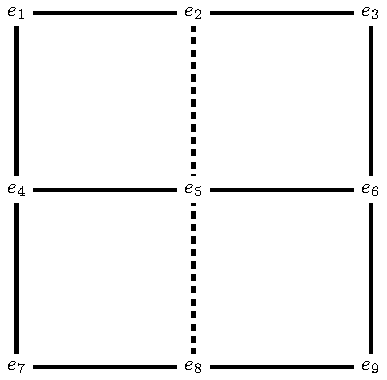
\includegraphics{MagicSquare-figure30.pdf}}
	    &
	    &\resizebox{0.3\textheight}{!}{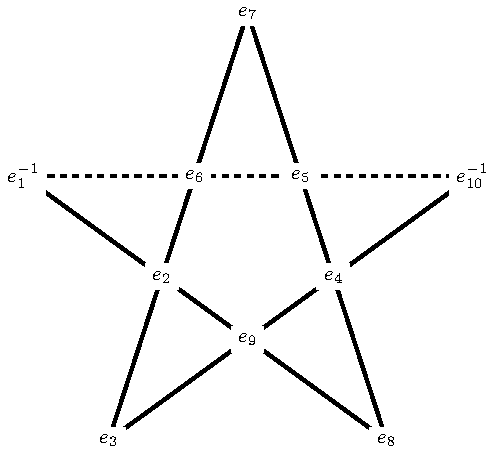
\includegraphics{MagicSquare-figure10.pdf}}
   	\end{tabular}
\caption{On the left-hand figure, the product of the generators on any solid line is equal to $1$ in the solution group of the magic square. The product of the operators on the dashed line is equal to $J$. Similarly, on the right-hand figure, the alternating product $ab\1cd\1$ is equal to $1$ on the solid lines and $J$ on the dashed line.}
	\label{fig:magic-game-generators}
\end{figure}

\begin{example}[Operator solution for magic pentagram]
See the pentagram of group generators in Figure \ref{fig:magic-game-generators}. Let $\G_3$ be the solution group of the Magic Pentagram. Consider the map $\G_3 \to U(\C^d\otimes \C^d\otimes\C^d)$ generated by sending each generator in this pentagram to the operator in the corresponding location of Figure \ref{fig:magic-square-operators-introduction}. This map is an operator solution.
\end{example}


\begin{prop}
\label{prop: perfect strategy}
	Let $\s: \G \to U(\C^D)$ be an operator solution. Define a strategy by setting $\ket\psi = \ket{\r{EPR}_D}$, $A_e^{(v)} = \s(e)$ for all $e,v,$ and $B_e = \bar{\s(e)}$ for all $e$. Provers using this strategy win with probability $1$.
\end{prop}
\begin{proof}
	By a well-known property of the maximally entangled state, we have
	\begin{equation}
		\braket{ \psi | \s(e) \otimes \bar{\s(e)} | \psi} = 
		\braket{ \psi | \s(e)\bar{\s(e)}^T \otimes I  | \psi} = 1,
	\end{equation}
	where $^T$ denotes the transpose. 
	Therefore, the consistency criterion \eqref{eq:exact-win-criterion-con} is satisfied.
	Since $\s$ is an operator solution, we have 
	\begin{align}
		\prod_{e} \left(A_e^{(v)}\right)^{H(v,e)} 
		\\&= \s(\prod_e \s(e)^{H(v,e)})
		\\&= \s(J^{l(v)}) 
		\\&=\w_d^{l(v)}I,
	\end{align}
	so the constraint satisfaction criterion \eqref{eq:exact-win-criterion-sat} is satisfied.
\end{proof}

We'll see both exact and approximate converses to this proposition in Section \ref{sec:self-testing}.
